% !TEX root = ../../thesis.tex

\newpage
\section{Extending the sensor apparatus of Poppy} % (fold)
\label{sec:morphology-adding-mechanism}

Poppy has been designed following a methodology (presented in section~\ref{REF}) which makes easy the hacking of the platform.
The last experiments presented mechanical modifications of Poppy's morphology. Indeed thanks to its 3D printed structure, it is quite easy and straightforward to modify its mechanical parts, unfortunately we cannot (yet) print complex electronics circuits and components.

We therefore chose design a custom I/O board based on Arduino (detailed in section~\ref{REF}). As its name suggests, this board has for main purpose to ensure the several inputs/outputs of the robot and offers:
\begin{itemize}
    \item 2 Dynamixel buses (TTL),
    \item 2 internal USB and 2 external USB ports,
    \item analog and digital pins available on a classic Arduino Due which can be use as direct input/output or for communication buses such as UART, I2C or SPI.
\end{itemize}
Thus there are many more I/Os than required for Poppy. These extra ports has been intended to let Poppy users extend its sensorimotor space and adapt it to their needs.


During our first trials to design walking a primitive with Poppy, we have been interested in the measurement of under feet pressures but the simple foot design Poppy had, does not involve such sensors. With a traditional robotic platform, we should have to either use the available sensors, here the load measurement in the ankle Dynamixel motor, or add an external device with its own power supply and communication system.

With the Poppy electronic modularity, we can hack the robot and integrate new sensors. Then they can be plugged on the I/O board for communication and power supply needs.

To provide an example of how we can actually hack the Poppy robot, we will explain here what we did to integrate force sensors under the feet and acquire the data with the pypot library.


\subsection{Integration of foot pressure sensors on Poppy} % (fold)

To obtain measurement of the pressure variation under our Poppy's feet we used FSR sensors from Interlink Electronics (see \figurename~\ref{fig:FSR_explode_view}). The FSR sensor will vary its resistance depending on how much pressure is being applied to the sensing area. The harder the force, the lower the resistance is. The acquisition of the FSR value require to create a simple voltage-divider those the design is explained in appendix \ref{appendix:design_FSR}. These sensors are low-cost -6\$ each- yet theirs behaviors are very non-linear (see \figurename~\ref{fig:foot_sensor_behavior}) and the calibration is quite variable depending on the production batch and the thermal conditions. So we cannot expect having precise results.

When we did the integration of foot sensors on the Poppy, its feet were still a really simple and flexible 3D printed part. The actual force transmission was done by the shoes. We therefore had to directly attach the sensors below the shoes.
To avoid multiple wires (2 per sensor) going from the head to the feet, we decided to use additional arduino nano boards to acquire sensors values of each foot and stream the data through serial communication up to the IO board.

Because Arduino nano board has 8 analog inputs, we have added 8 sensors under each foot (see \figurename~\ref{fig:poppy_foot_sensors}) but actually only used 5 (the big ones) and integrated the arduino nano in the leg. While it was a hack of a real shoe and not just a print of new part, the intervention was quite annoying but still achievable in one day. Here we have chosen to use USB cable to plug each Arduino nano in the Poppy's head but it could also have be done using UART, SPI or I2C communication.

\begin{figure}[h]
\centering
    \subfloat[][]{\label{fig:poppy_foot_sensors}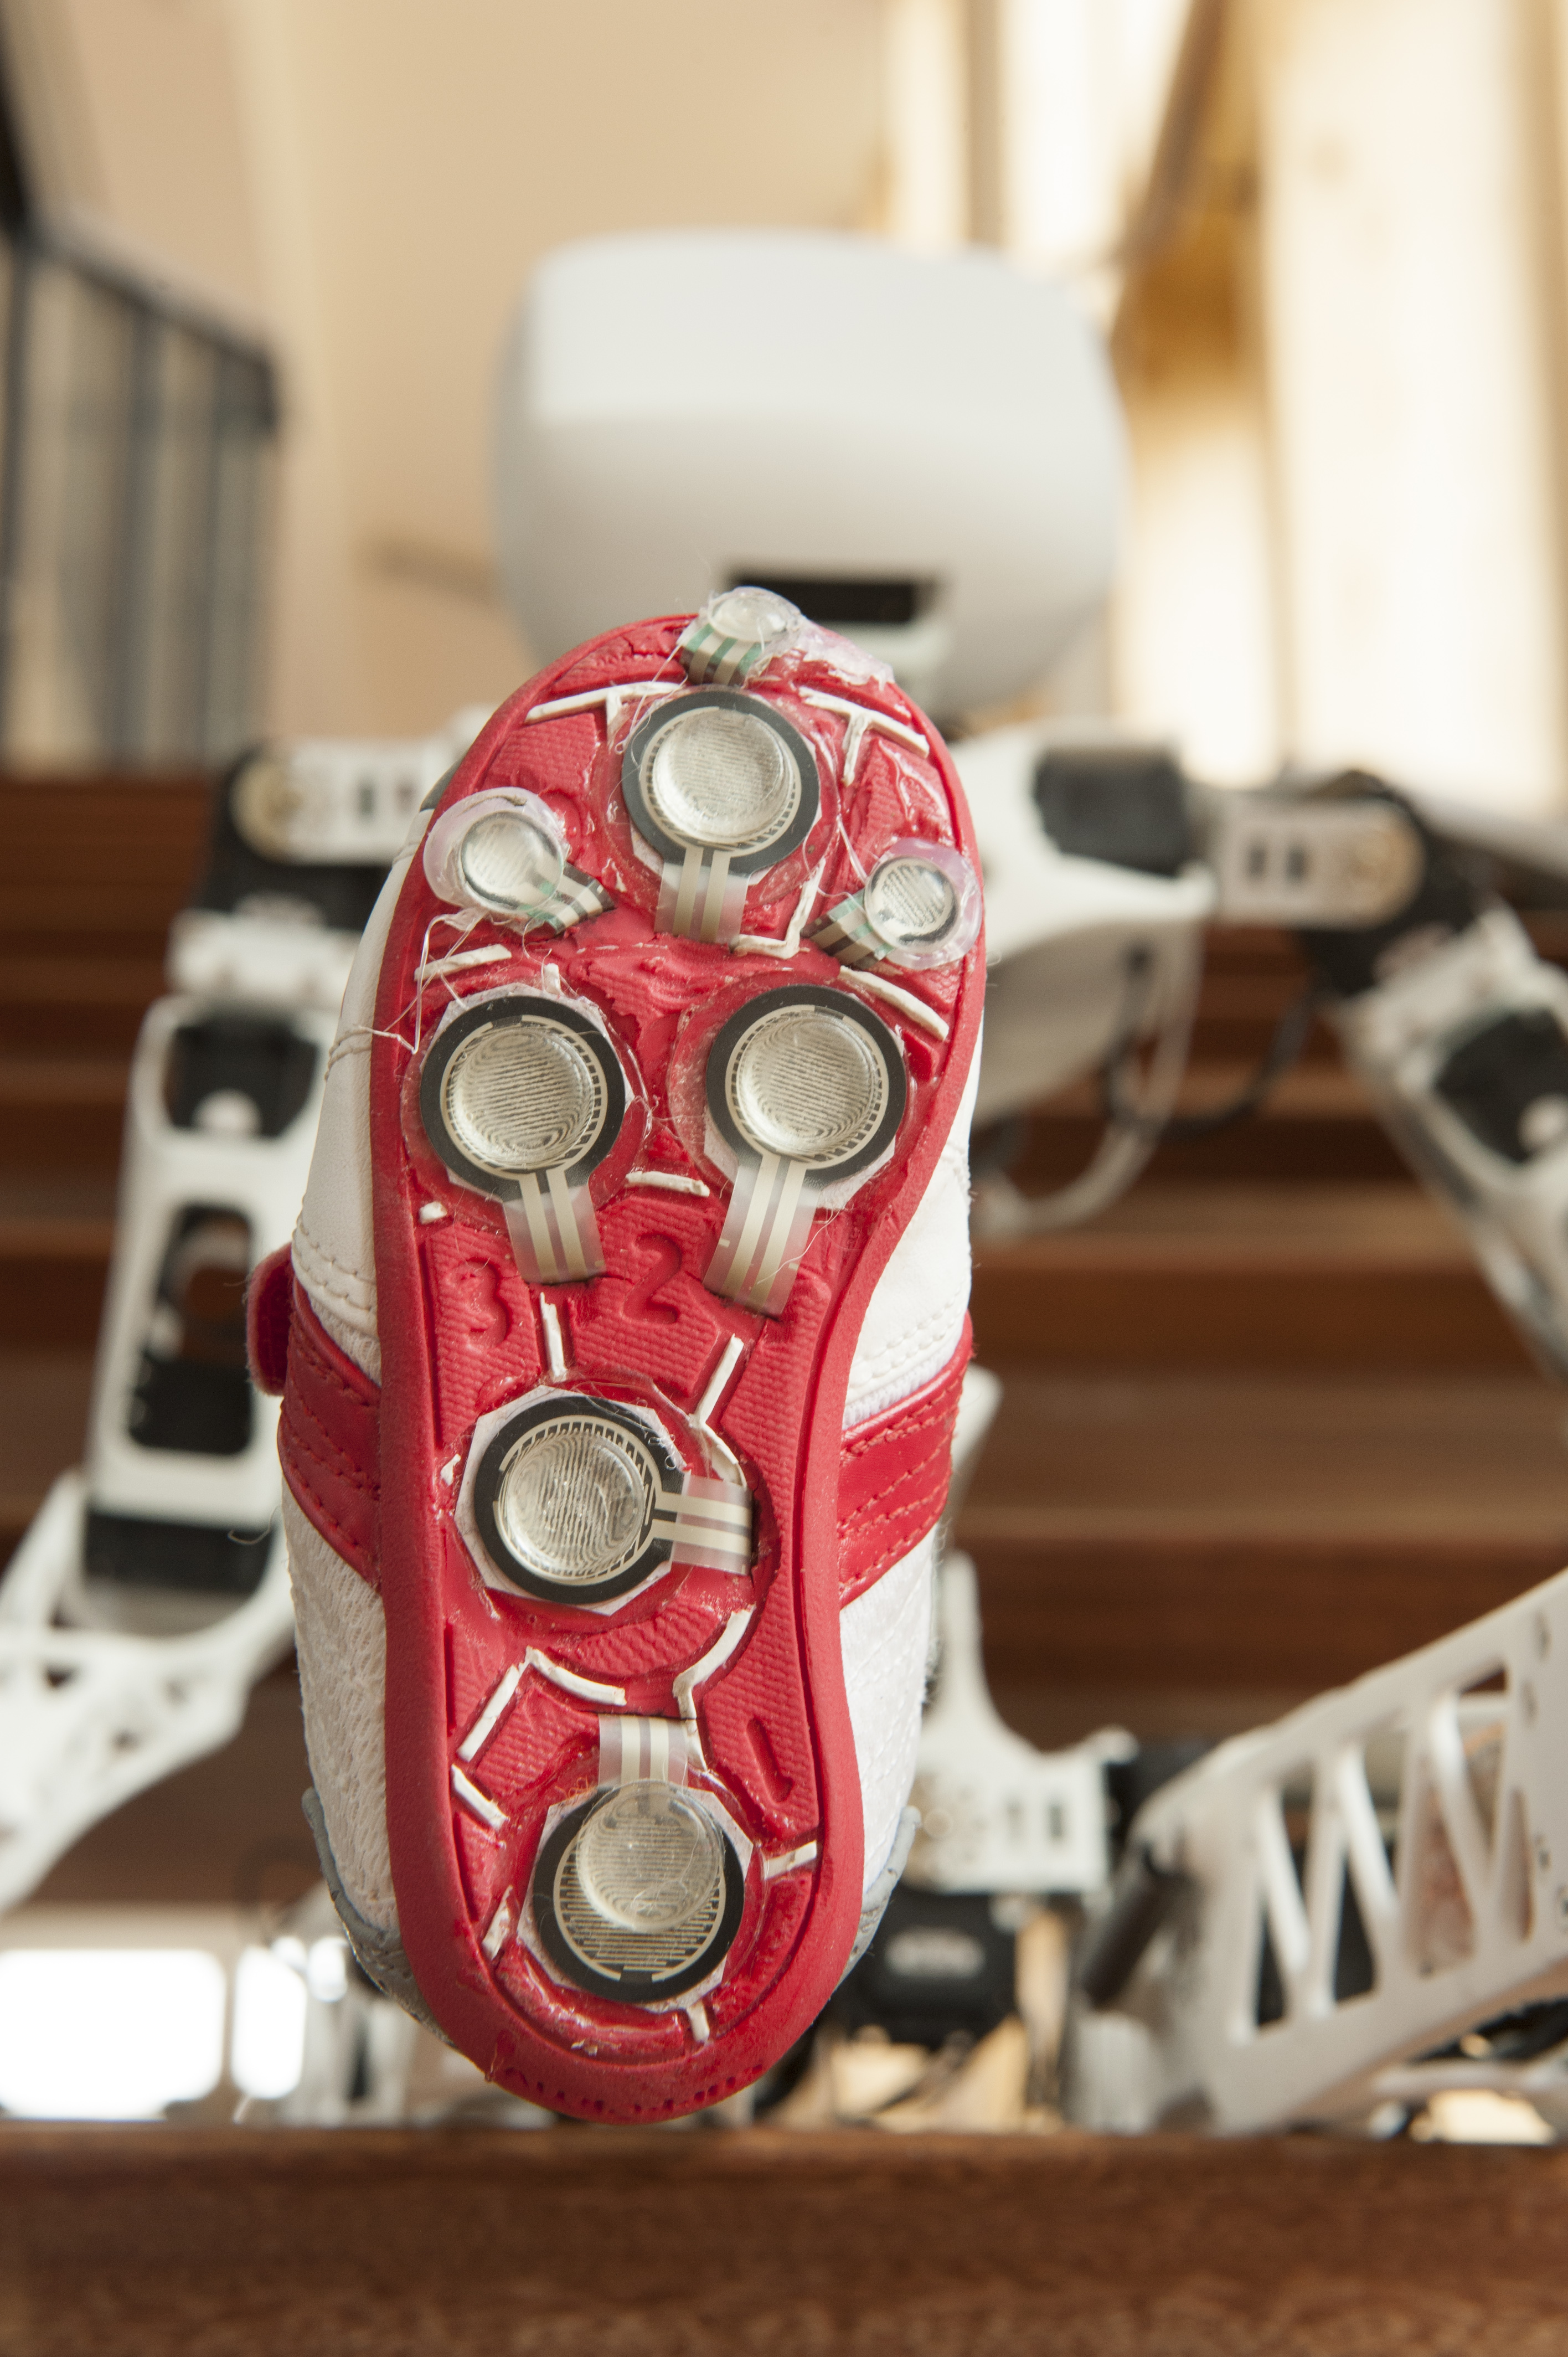
\includegraphics[height=7cm]{foot_sensors.jpg}}
    \hfil
    \subfloat[][]{\label{fig:poppy_nano_integration}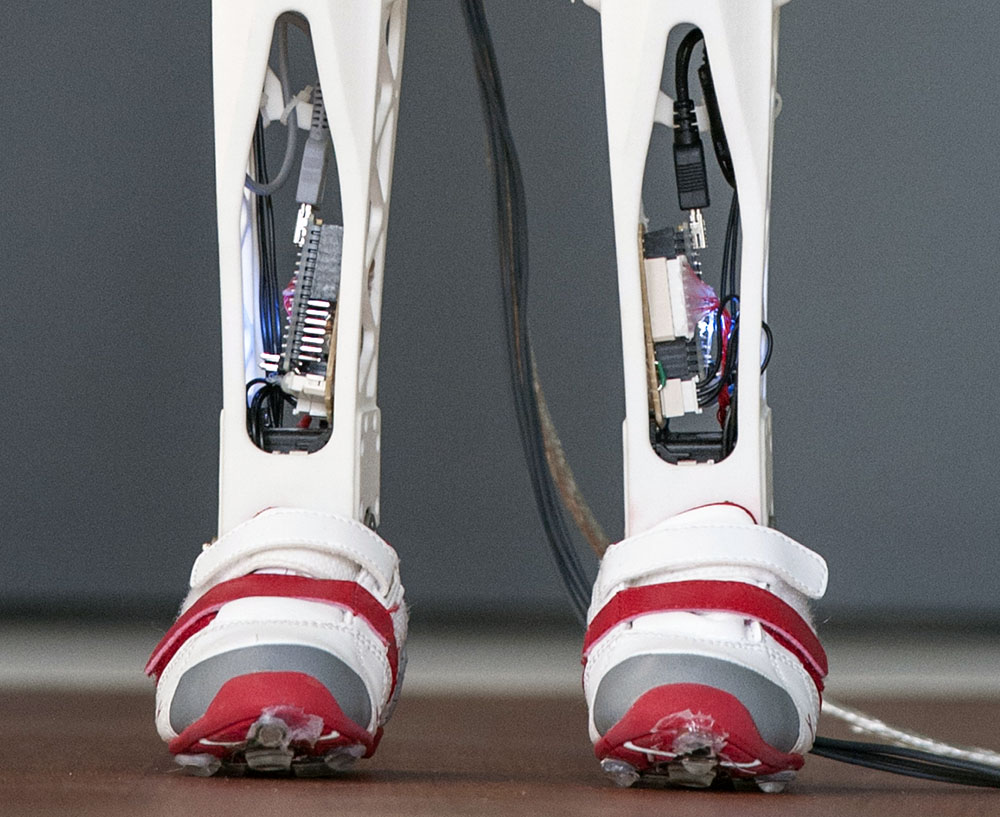
\includegraphics[height=7cm]{poppy_leg_arduino_nano.jpg}}
    \caption{}
    \label{fig:poppy_foot_sensors}
\end{figure}


As we explained in section~\ref{REF}, the Arduino programming language bring the low level programming accessible to anyone. The \codename~\ref{code:arduino_foot_sensor} shows that we actually uploaded on each Arduino nano board. With just 10 lines of code we can stream the values of 5 pressure sensors.

\lstinputlisting[
    language = C++,
    caption = {Arduino code to read force sensors data},
    label = {code:arduino_foot_sensor},
    float,
    floatplacement = H]
    {code/foot_force_sensors.ino}

Then we just have to create a novel sensor controller in pypot (see section~\ref{REF} for details) which describes the I/O communication and get the desired values (see \codename~\ref{code:pypot_foot_sensor}). Here again, the design of the pypot library makes this task easy, only 20 lines of code are required to get access to add a novel sensor and create variable to obtain its value.

\lstinputlisting[
    language = Python,
    caption = {Example of Python code written to add custom foot sensors in pypot. The \emph{FootIO} class describes how we can read the data from the Arduino nano placed in the foot. The \emph{FootPressure} class is the sensor controller which is called by the pypot to synchronize the sensorimotor space of Poppy.},
    label = {code:pypot_foot_sensor},
    float,
    floatplacement = H]
    {code/foot_io.py}


\subsection{Measured data} % (fold)
With our novel sensors, we conducted similar walking experiment as the one explains in section~\ref{REF} and shows on the \figurename~\ref{fig:humanoids2013_cpg_on_poppy} and recorded at $50hz$ the measured force variations under Poppy's feet.

The sensors are not very precise but as we can see on \figurename~\ref{fig:poppy_GRF}, the variation of the ground reaction force (mean of the 5 force sensors) over the gait cycle has a similar M-shape as the one we can find in human gait (see \figurename~\ref{fig:human_GRF}). Also we can notice than the reaction is slightly different between the two foot (\figurename~\ref{fig:right_GRF} Vs \figurename~\ref{fig:left_GRF}).

\begin{figure}[!h]
\centering
    \subfloat[][]{\label{fig:right_GRF}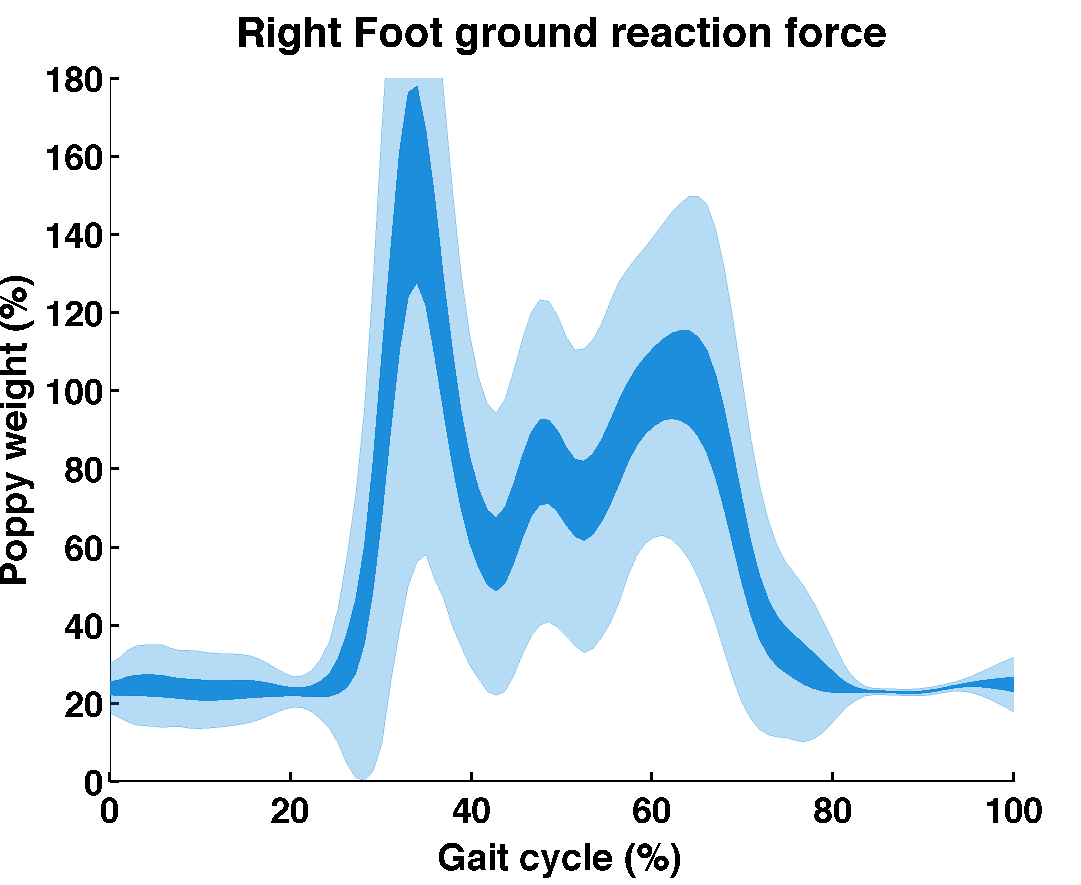
\includegraphics[width=0.48\linewidth]{right_GRF.pdf}}
    \hfil
    \subfloat[][]{\label{fig:left_GRF}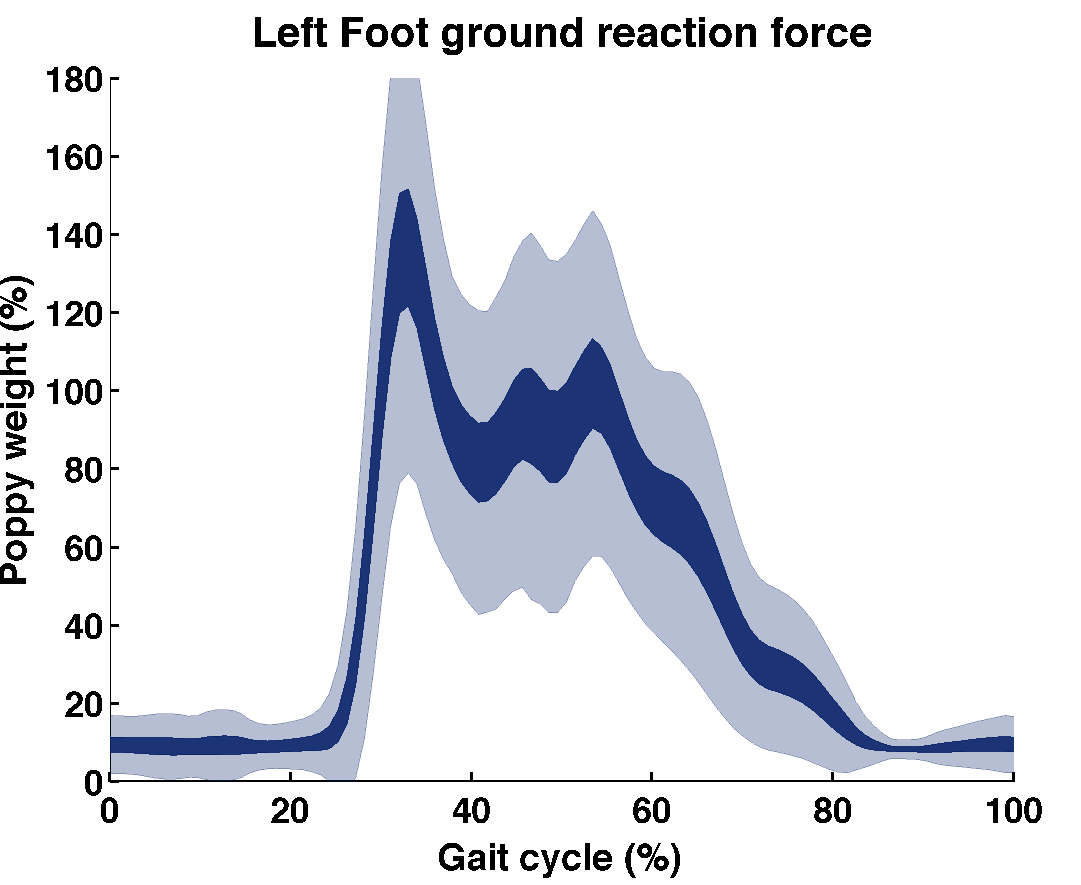
\includegraphics[width=0.48\linewidth]{left_GRF.pdf}}
    \caption{}
    \label{fig:poppy_GRF}
\end{figure}


\begin{figure}[!h]
\centering
    \subfloat[][]{\label{fig:}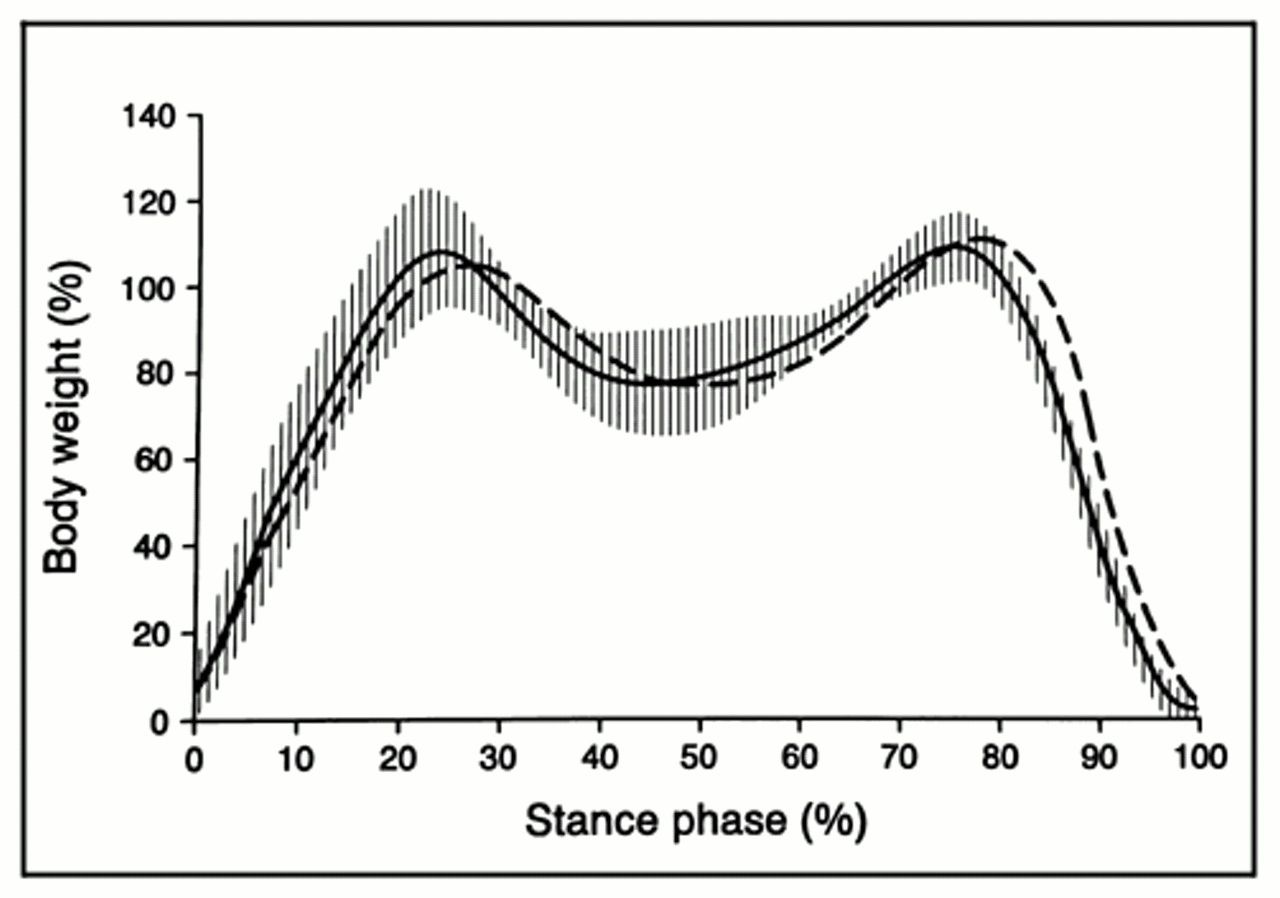
\includegraphics[width=0.3\linewidth]{human_GRF.jpg}}
    \hfil
    \subfloat[][]{\label{fig:}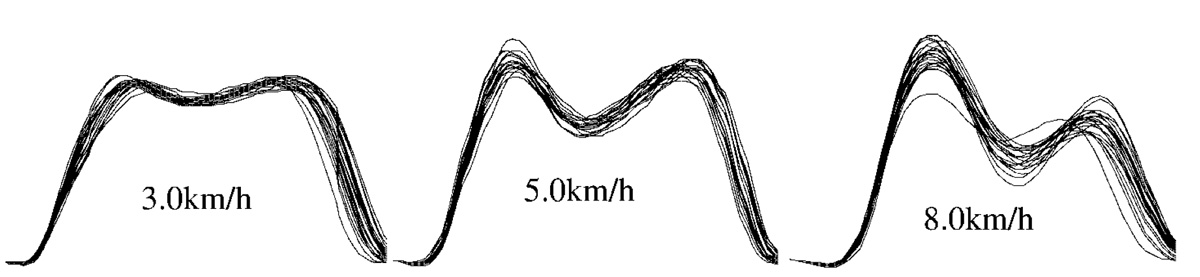
\includegraphics[width=0.7\linewidth]{human_GRF_variation.jpg}}
    \caption{}
    \label{fig:human_GRF}
\end{figure}


The bad precision of the sensors prevents us from affirming conclusions but it can still give insights to understand the walking behavior of Poppy:
\begin{enumerate}
    \item The second peak of the M-shape corresponding to the toe impulsion is weak or inexistent on Poppy. Indeed, when we look at the video of the walking gait made by Poppy, we can notice it barely uses its toes.
    \item The first peak of the M-shape is very strong. Either the walking gait of Poppy was fast or the structure is too rigid and does not absorb correctly the initial impact.
\end{enumerate}

We can therefore explore some improvements axes:
\begin{enumerate}
    \item Explore why the current walking behavior does not involve clearly the passive toes. Is it cause of the walking primitive design or the mechanical design of the toes ?
    \item The initial impact is not desirable toward the achievement of a self-balanced walking behavior. We should explore solutions to absorb it.
\end{enumerate}







